\section{Lecture 4: Independent Component Analysis}

Independent Component Analysis (ICA) returns to the projection-method theme from PCA, but it changes the question. PCA asks for directions that explain second-order variance. ICA asks for directions that recover the latent causes whose signals were mixed together before measurement.

The mental model is the cocktail party problem. Several acoustic sources are active at the same time, several microphones record different weighted sums of those sources, and the task is to recover the original source signals without knowing the mixing weights in advance. The same abstraction appears in EEG, where sensor traces can contain mixtures of neural activity, eye blinks, muscle artifacts, and line noise.

ICA is therefore a bridge between three earlier course ideas:
\begin{itemize}
  \item like PCA, it is a linear projection method;
  \item like Hebbian learning, it can be implemented by an online neural learning rule;
  \item like HMMs, it is a latent-variable model whose useful structure is not directly observed.
\end{itemize}
The new ingredient is the statistical prior. PCA uses uncorrelatedness and variance. ICA uses statistical independence and non-Gaussianity.

\subsection{Blind Source Separation}

The problem solved by blind source separation is that the observation coordinates are not the meaningful coordinates. A microphone, electrode, or sensor channel is often a mixture of several physical causes. If the causes are independent, then the right coordinate system should make the recovered coordinates statistically independent rather than merely uncorrelated.

Let
\[
  s =
  \begin{bmatrix}
    s_1\\ \vdots\\ s_N
  \end{bmatrix}
  \in \mathbb{R}^N
\]
be the latent source vector at one time point. The component \(s_i\) is the activity of source \(i\). Its numerical value measures the instantaneous amplitude of that source. Across time or samples, its distribution describes how often that source takes different amplitudes.

The observed vector is
\[
  x =
  \begin{bmatrix}
    x_1\\ \vdots\\ x_N
  \end{bmatrix}
  \in \mathbb{R}^N.
\]
The component \(x_j\) is the measurement at sensor \(j\). It is not assumed to be a single source. In the simplest ICA model it is a linear superposition:
\[
  x = A s.
\]
Here \(A\in\mathbb{R}^{N\times N}\) is the mixing matrix. Column \(a_i\) of \(A\) is the sensor-space pattern induced by source \(s_i\). If \(s_i\) changes while all other sources are held fixed, \(x\) moves in direction \(a_i\).

The aim is to learn an unmixing matrix
\[
  W\in\mathbb{R}^{N\times N}
\]
so that
\[
  \hat{s}=Wx
\]
is a vector of recovered source signals. Row \(w_i^{\mathsf{T}}\) of \(W\) is a spatial filter: it takes the observed mixture \(x\) and returns the estimated source amplitude \(\hat{s}_i=w_i^{\mathsf{T}}x\).

\begin{figure}[htbp]
  \centering
  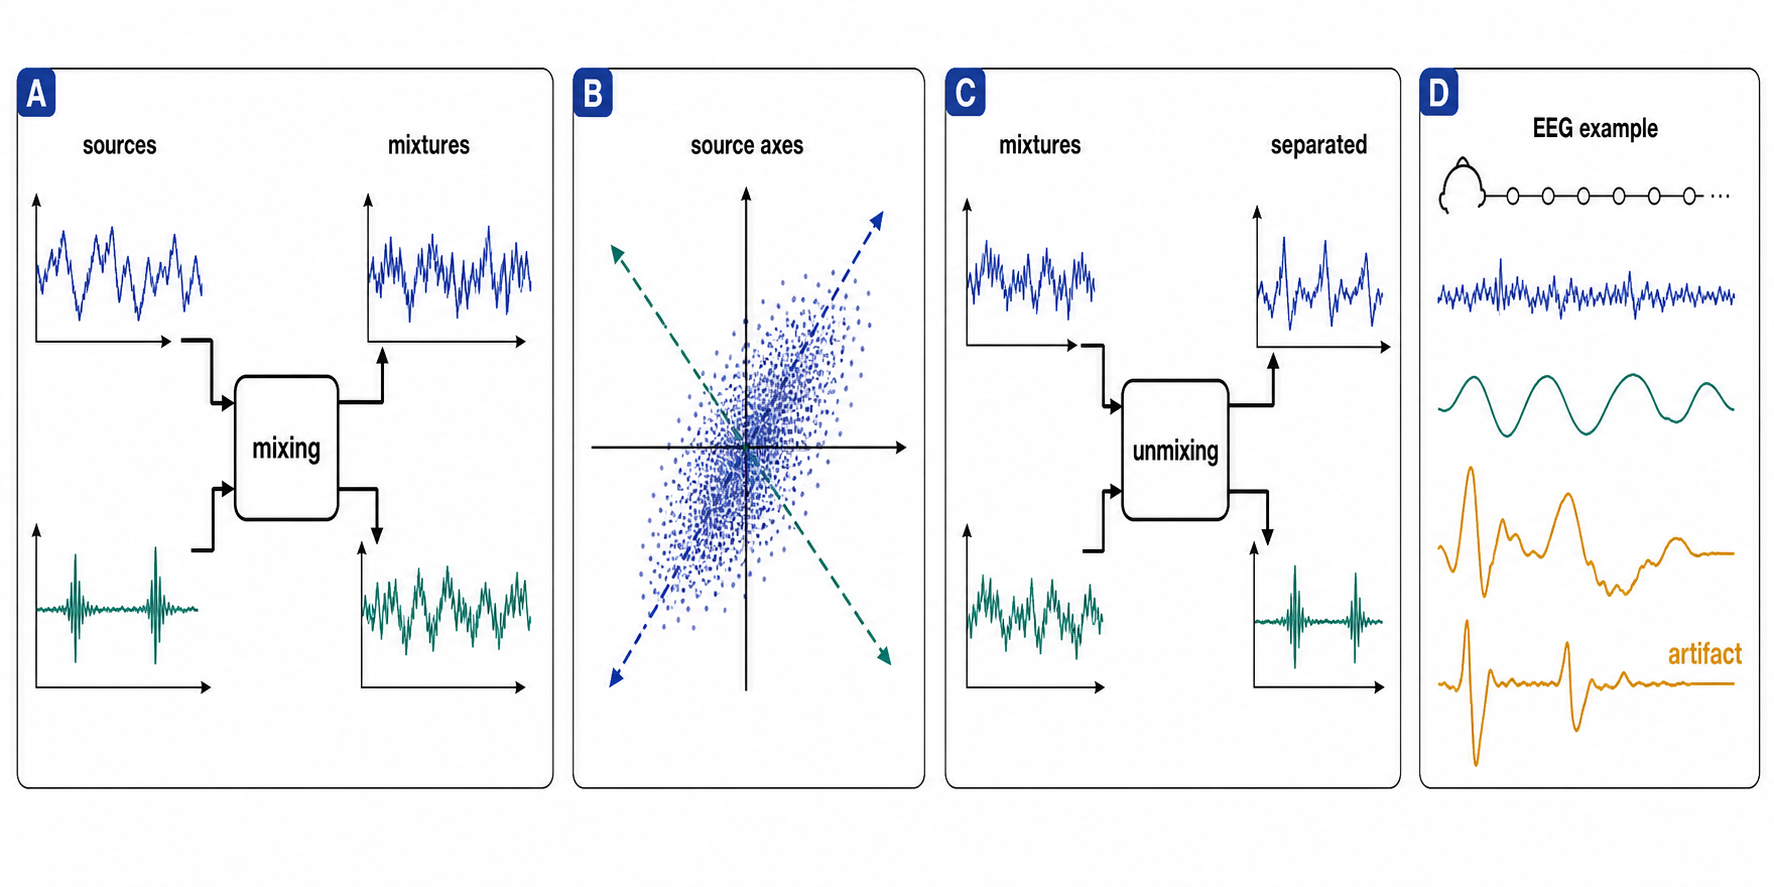
\includegraphics[width=0.96\textwidth]{figures/ica/bss-unmixing.png}
  \caption{ICA as blind source separation. Latent source signals are mixed by the unknown matrix \(A\), producing observed mixtures \(x\). The learned unmixing matrix \(W\) tries to recover source coordinates \(\hat{s}\). In EEG-like settings, this can separate neural components from stereotyped artifacts, but the recovered components still require interpretation.}
\end{figure}

For two sources,
\[
  A =
  \begin{bmatrix}
    a_{11} & a_{12}\\
    a_{21} & a_{22}
  \end{bmatrix},
  \qquad
  x =
  \begin{bmatrix}
    a_{11}s_1+a_{12}s_2\\
    a_{21}s_1+a_{22}s_2
  \end{bmatrix}.
\]
If \(s=(1,0)^{\mathsf{T}}\), then \(x=a_1\), the first column of \(A\). If \(s=(0,1)^{\mathsf{T}}\), then \(x=a_2\), the second column of \(A\). Thus the source axes appear as oblique directions in observation space. PCA can rotate the cloud into uncorrelated axes, but those axes need not coincide with the source directions.

\paragraph{Why prior knowledge is necessary.}
Suppose we observe \(p\) samples \(x^{(\alpha)}\), \(\alpha=1,\dots,p\). The data contain \(pN\) observed numbers. If both \(A\) and the entire source sequence \(s^{(\alpha)}\) are unknown, the model contains \(N^2+pN\) unknown numbers. Without an additional constraint, many different source sequences and mixing matrices can explain the same observations. ICA becomes identifiable only because it assumes that the source coordinates are statistically independent and not all Gaussian.

\paragraph{Practical implication.}
When using ICA, first ask whether independent sources are a plausible measurement model. ICA is not just a rotation trick. It encodes the claim that the observed channels combine distinct causes whose joint density factorizes in the correct coordinates.

\subsection{Independence Is Stronger Than Decorrelation}

The problem with PCA as a source-separation method is that covariance is only a second-order summary. PCA can remove linear correlations, but independence is a statement about the full joint distribution.

For centered random variables \(y_i\) and \(y_j\), decorrelation means
\[
  \mathbb{E}[y_i y_j]=0.
\]
This says that the covariance matrix is diagonal in the chosen coordinate system. It does not rule out nonlinear dependence. Two variables can be uncorrelated while one still predicts the magnitude, sign pattern, or tail probability of the other.

Independence means
\[
  p_y(y)
  =
  \prod_{i=1}^{N}p_{y_i}(y_i),
\]
where \(p_y\) is the joint density of the vector \(y\), and \(p_{y_i}\) is the one-dimensional marginal density of coordinate \(i\). This factorization says that knowing one coordinate changes nothing about the distribution of the others. It is a full-density statement, not a covariance statement.

The usual ICA preprocessing pipeline uses PCA as a first step:
\begin{enumerate}
  \item center the data, so the sample mean is zero;
  \item diagonalize the covariance matrix \(C_x=M\Lambda M^{\mathsf{T}}\);
  \item whiten the observations with
  \[
    z=\Lambda^{-1/2}M^{\mathsf{T}}x.
  \]
\end{enumerate}
The whitened vector \(z\) has covariance
\[
  \mathbb{E}[zz^{\mathsf{T}}]=I.
\]
Whitening removes scale and covariance structure. If the true sources have been scaled to unit variance, then the remaining ICA problem is mostly rotational: find the rotation in whitened space whose coordinates are independent.

\begin{figure}[htbp]
  \centering
  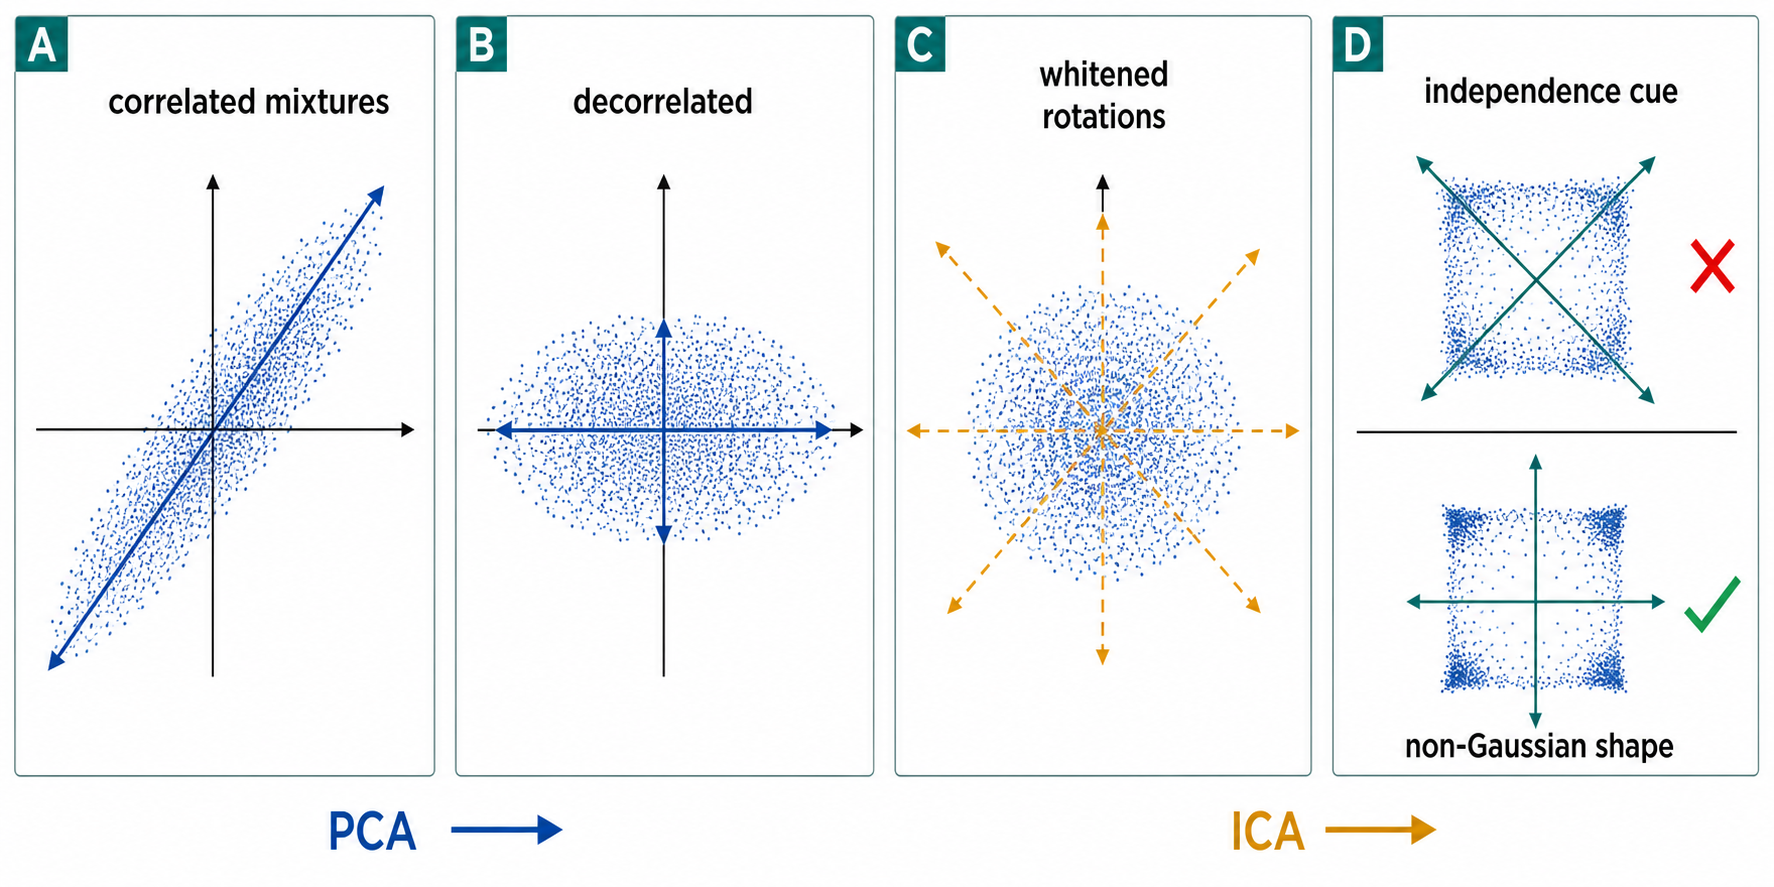
\includegraphics[width=0.96\textwidth]{figures/ica/whitening-nongaussianity.png}
  \caption{Decorrelation is not independence. PCA rotates the data to remove covariance, whitening rescales the coordinates to unit variance, and ICA still has to choose among the remaining rotations. Non-Gaussian shape supplies the cue that covariance alone cannot provide.}
\end{figure}

The non-Gaussian cue is visible in simple two-dimensional examples. If two independent sources have a square-like, sparse, or heavy-tailed joint cloud after mixing and whitening, only some rotations align with the edges, spikes, or tail directions of that cloud. ICA uses those high-order distributional features to choose the source axes.

\paragraph{Practical implication.}
Whitening is not a replacement for ICA. It is a conditioning step that removes the part of the problem already solved by PCA. After whitening, inspect what remains: if all rotations look statistically similar, the data may not contain enough non-Gaussian structure for reliable source separation.

\subsection{Identifiability Limits}

The problem solved by identifiability analysis is to separate what ICA can learn from what no algorithm can learn. Even with perfect data and perfect optimization, the recovered sources have unavoidable ambiguities.

\subsubsection{Permutation Ambiguity}

If \(P\) is a permutation matrix, then
\[
  x = A s = A P^{\mathsf{T}} P s.
\]
The transformed source vector \(\tilde{s}=Ps\) contains the same source signals in a different order, and the transformed mixing matrix \(\tilde{A}=A P^{\mathsf{T}}\) gives the same observations. Therefore ICA cannot determine which recovered component should be called source \(1\), source \(2\), and so on.

This ambiguity is harmless for separation but important for evaluation. Matching recovered components to ground-truth components requires a best permutation, not coordinatewise comparison in the original order.

\subsubsection{Scale Ambiguity}

If \(D\) is an invertible diagonal matrix, then
\[
  x = A s = A D^{-1} D s.
\]
The transformed source vector \(\tilde{s}=Ds\) rescales each source, while \(\tilde{A}=AD^{-1}\) compensates in the mixing matrix. Observations do not determine source amplitudes absolutely. A component can be twice as large if the corresponding mixing column is half as large.

In practice, ICA algorithms impose a convention, for example unit variance sources, fixed diagonal entries of \(W\), or normalized rows of \(W\). These conventions stabilize learning, but they are not source facts.

\subsubsection{Gaussian Rotation Ambiguity}

Gaussian sources are the deeper limit. If
\[
  s\sim\mathcal{N}(0,I),
\]
then the density is
\[
  p_s(s)
  =
  \frac{1}{(2\pi)^{N/2}}
  \exp\left(-\frac{1}{2}\|s\|^2\right).
\]
For any orthogonal matrix \(B\) with \(B^{\mathsf{T}}B=I\),
\[
  \|Bs\|^2
  =
  s^{\mathsf{T}}B^{\mathsf{T}}Bs
  =
  \|s\|^2.
\]
Thus \(Bs\) has the same standard Gaussian density as \(s\). Rotations of a spherical Gaussian are statistically indistinguishable. If all sources are Gaussian, no density-based method can identify the source axes after whitening.

\begin{figure}[htbp]
  \centering
  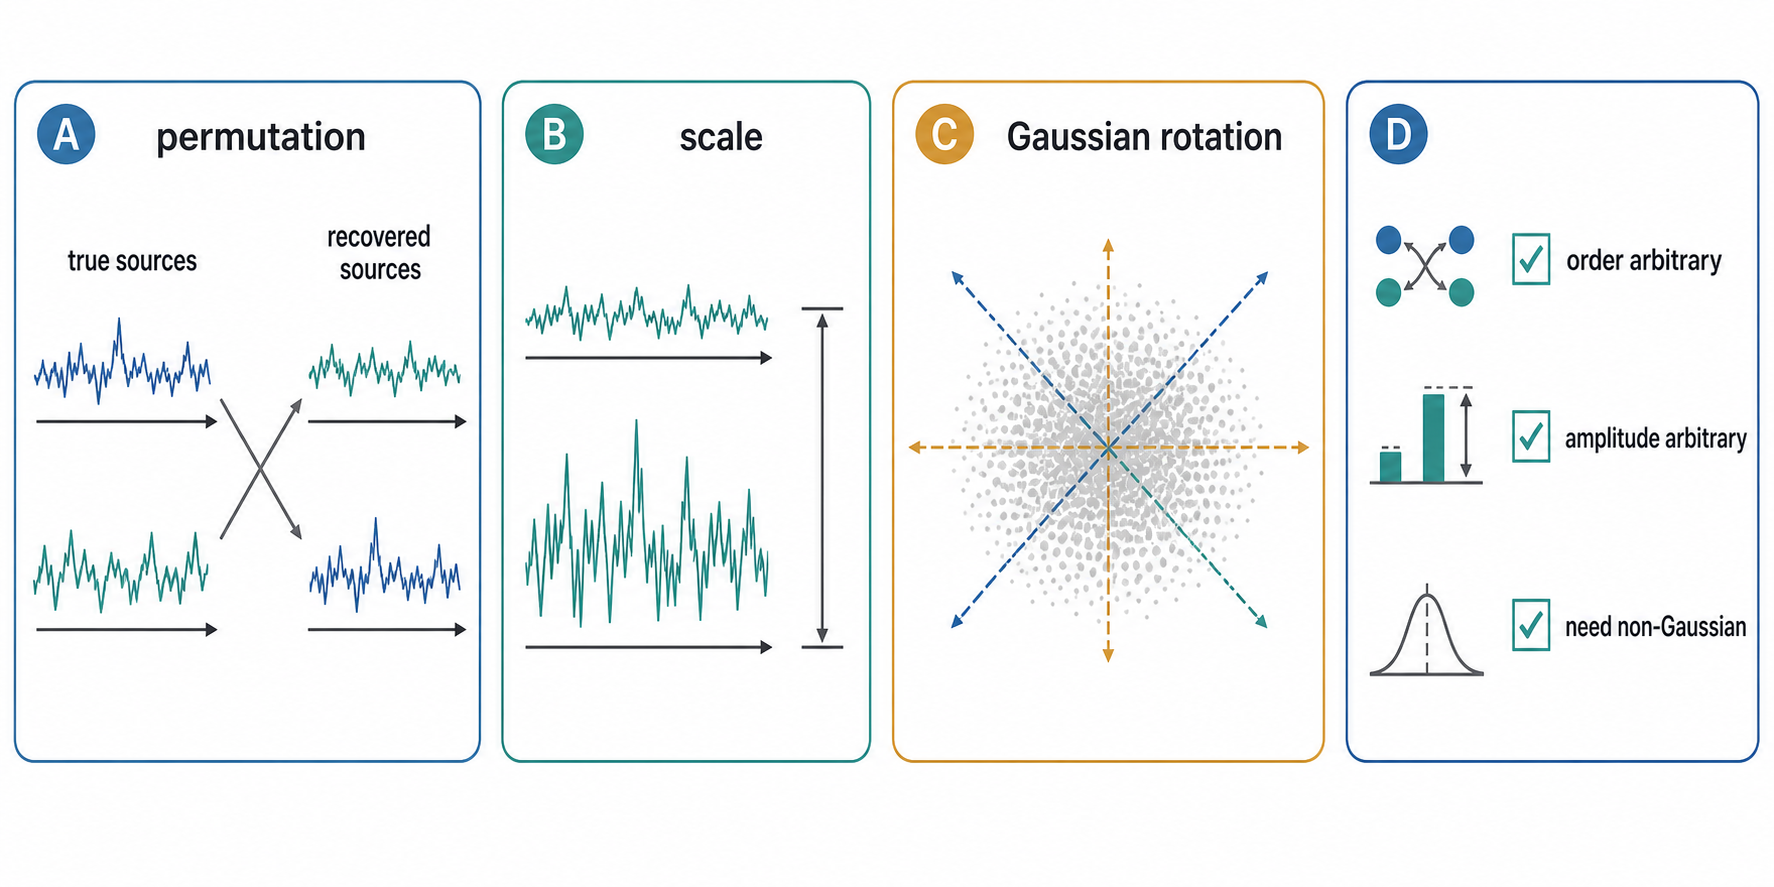
\includegraphics[width=0.96\textwidth]{figures/ica/identifiability-limits.png}
  \caption{ICA has unavoidable identifiability limits. The order of recovered sources is arbitrary, their amplitudes require a convention, and Gaussian sources do not reveal a preferred rotation because a spherical Gaussian looks the same from every orthogonal coordinate system.}
\end{figure}

The usual identifiability statement is: under the linear instantaneous mixing model, independent sources can be recovered up to permutation and scale if at most one source is Gaussian and the mixing matrix is invertible.

\paragraph{Practical implication.}
Do not interpret component index or raw component amplitude as meaningful without an external convention. Interpret the shape, time course, mixing pattern, and reproducibility of a component instead.

\subsection{Mutual Information As The Independence Objective}

The problem solved by an ICA objective is model selection. Among many possible matrices \(W\), choose the one whose recovered coordinates are closest to statistically independent.

Let
\[
  \hat{s}=Wx
\]
be the recovered source vector. The density \(p_{\hat{s}}(\hat{s})\) is the true density induced by the data and the current \(W\). ICA compares it to the factorized model
\[
  q_{\hat{s}}(\hat{s})
  =
  \prod_{i=1}^{N}p_{\hat{s}_i}(\hat{s}_i),
\]
which keeps each one-dimensional marginal but removes all dependence between coordinates.

\begin{figure}[htbp]
  \centering
  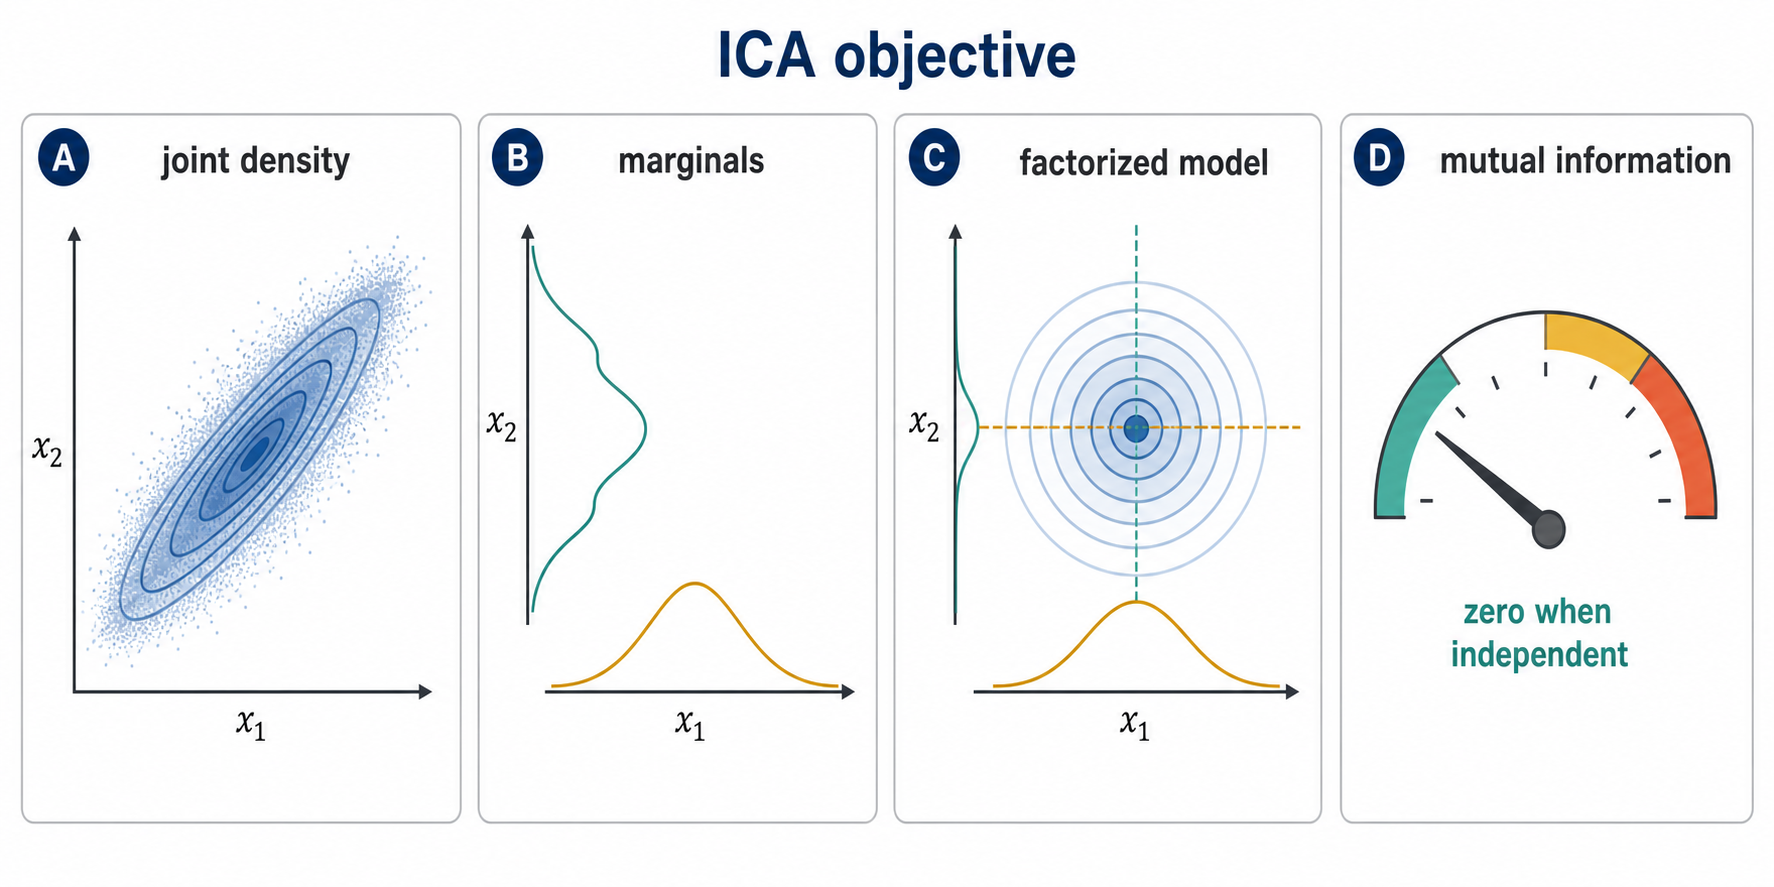
\includegraphics[width=0.96\textwidth]{figures/ica/mutual-information-factorization.png}
  \caption{Mutual information as residual dependence. ICA compares the recovered joint density with the factorized density formed from its one-dimensional marginals. The KL gap is zero only when the recovered coordinates are independent, so minimizing mutual information selects the unmixing coordinates that remove dependence.}
\end{figure}

The Kullback--Leibler divergence from the true joint density to this factorized density is
\[
  D_{\mathrm{KL}}
  \left(
    p_{\hat{s}}
    \,\middle\|\,
    \prod_{i=1}^{N}p_{\hat{s}_i}
  \right)
  =
  \int
  p_{\hat{s}}(\hat{s})
  \ln
  \frac{p_{\hat{s}}(\hat{s})}{
    \prod_{i=1}^{N}p_{\hat{s}_i}(\hat{s}_i)
  }
  \,d\hat{s}.
\]
This quantity is also the mutual information among the recovered coordinates. It is zero exactly when the joint density factorizes. ICA can therefore be written as
\[
  W^*
  =
  \operatorname*{arg\,min}_{W}
  I(\hat{s}_1,\dots,\hat{s}_N).
\]

Entropy gives another view. The differential entropy of a density \(p_y\) is
\[
  H(y)
  =
  -\int p_y(y)\ln p_y(y)\,dy.
\]
It measures distributional spread in continuous space. With this notation,
\[
  I(\hat{s}_1,\dots,\hat{s}_N)
  =
  \sum_{i=1}^{N}H(\hat{s}_i)
  -
  H(\hat{s}).
\]
The first term sums the marginal uncertainties. The second term is the joint uncertainty. If the coordinates are independent, the joint uncertainty equals the sum of marginal uncertainties and the mutual information is zero. If dependencies remain, the joint uncertainty is smaller than the sum of marginals, and the difference measures the redundancy.

\paragraph{Practical implication.}
ICA is not minimizing reconstruction error. If \(W\) is invertible, reconstruction can be exact for many \(W\). ICA chooses among those invertible representations by asking which one removes dependence between coordinates.

\subsection{The Infomax Principle}

The Infomax method solves the independence problem by transforming recovered sources through nonlinear output functions and maximizing the entropy of the outputs. The mental model is simple: if each source coordinate is passed through its own cumulative distribution function, then each output becomes uniformly distributed. Independent uniform outputs fill the output volume without redundancy, so their entropy is maximal.

For each recovered source coordinate \(\hat{s}_i\), introduce a strictly monotone nonlinearity
\[
  \hat{u}_i=\hat{f}_i(\hat{s}_i).
\]
The variable \(\hat{u}_i\) is the output of the ICA neuron after the nonlinearity. The function \(\hat{f}_i\) is chosen or learned to approximate a cumulative distribution function.

The conservation-of-probability argument is one-dimensional. For a monotone transformation \(\hat{u}_i=\hat{f}_i(\hat{s}_i)\),
\[
  p_{\hat{u}_i}(\hat{u}_i)\,d\hat{u}_i
  =
  p_{\hat{s}_i}(\hat{s}_i)\,d\hat{s}_i.
\]
Since
\[
  d\hat{u}_i
  =
  \hat{f}_i'(\hat{s}_i)d\hat{s}_i,
\]
we have
\[
  p_{\hat{u}_i}(\hat{u}_i)
  =
  \frac{p_{\hat{s}_i}(\hat{s}_i)}{\hat{f}_i'(\hat{s}_i)}.
\]
If the output density is required to be uniform with value \(1\) on its support, then
\[
  \hat{f}_i'(\hat{s}_i)=p_{\hat{s}_i}(\hat{s}_i),
\]
and therefore
\[
  \hat{f}_i(\hat{s}_i)
  =
  \int_{-\infty}^{\hat{s}_i}
  p_{\hat{s}_i}(y)\,dy.
\]
Thus \(\hat{f}_i\) is the cumulative distribution function of \(\hat{s}_i\).

The full Infomax network is
\[
  \hat{s}=Wx,
  \qquad
  \hat{u}_i=\hat{f}_i(w_i^{\mathsf{T}}x).
\]
The Infomax objective is
\[
  H(\hat{u})
  =
  -\int p_{\hat{u}}(\hat{u})\ln p_{\hat{u}}(\hat{u})\,d\hat{u}
  \quad \longrightarrow \quad \max_W.
\]
Maximizing this entropy encourages the output variables to use the available output volume with minimal redundancy.

\begin{figure}[htbp]
  \centering
  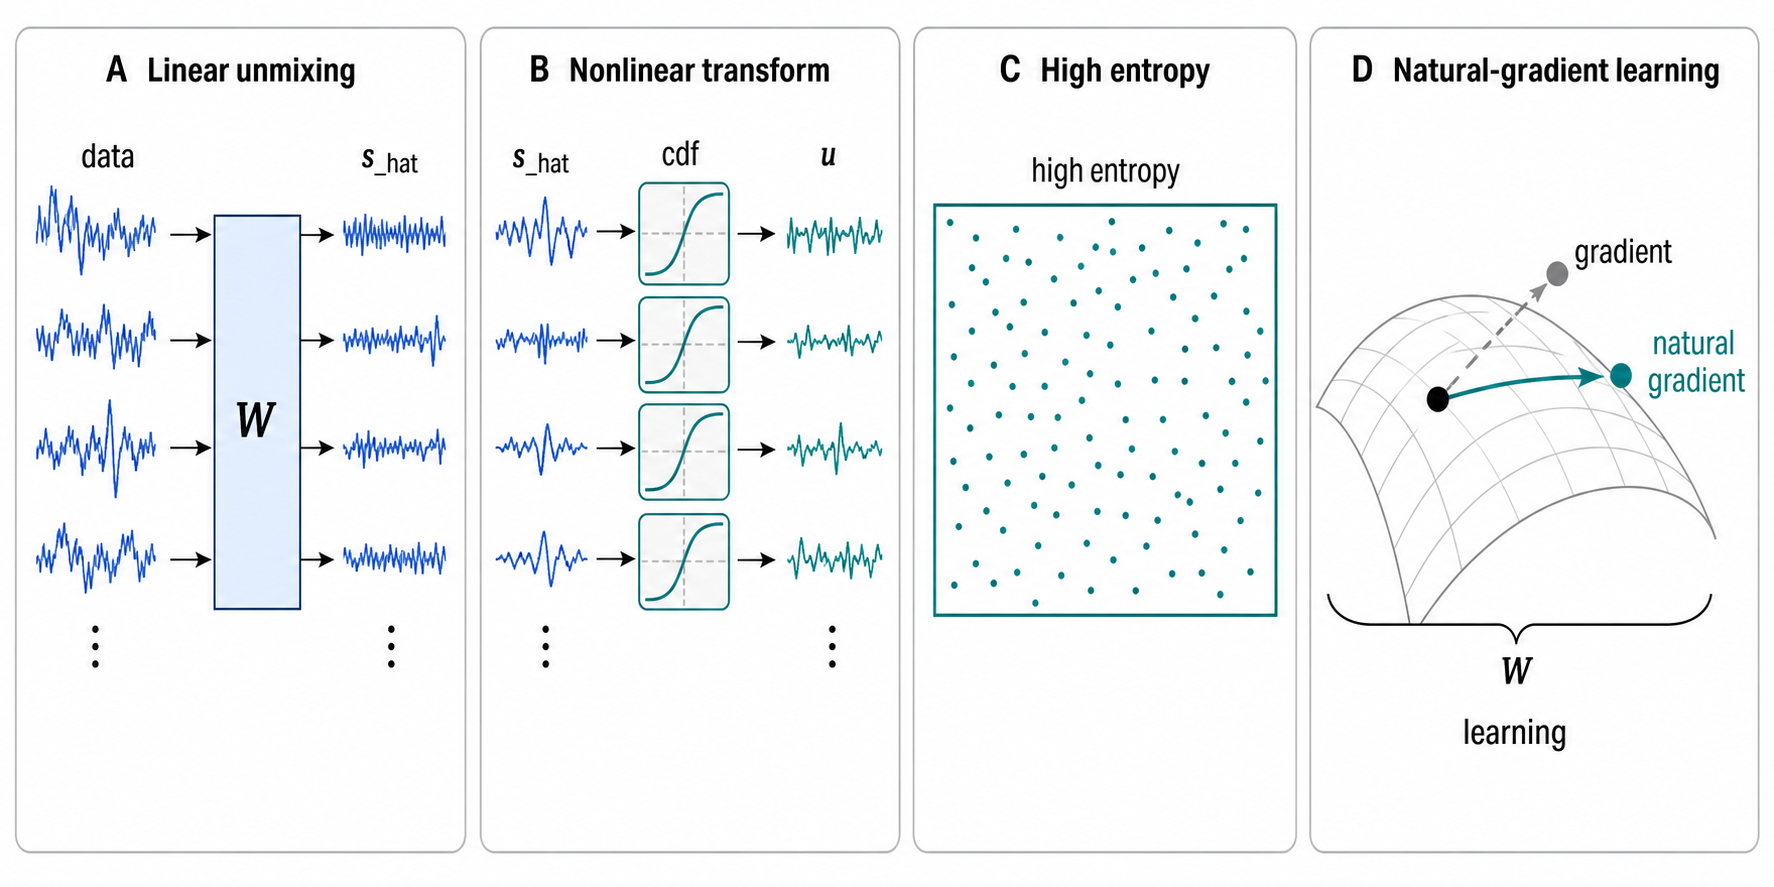
\includegraphics[width=0.96\textwidth]{figures/ica/infomax-natural-gradient.png}
  \caption{The Infomax ICA pipeline. A linear unmixing layer \(W\) produces estimated sources \(\hat{s}\), componentwise nonlinearities map them to output variables \(\hat{u}\), and maximizing output entropy supplies the learning objective. Natural-gradient learning adjusts the step to the geometry of invertible linear transforms.}
\end{figure}

\subsection{Deriving The Empirical Infomax Objective}

The problem solved by the empirical objective is that \(H(\hat{u})\) is a population quantity, but training uses samples. The derivation also explains why the determinant of \(W\) appears.

For one sample \(x\), define
\[
  y = Wx,
  \qquad
  u_i = f_i(y_i).
\]
The Jacobian of the full transformation \(x\mapsto u\) is
\[
  J(x)
  =
  \operatorname{diag}
  \bigl(
    f_1'(y_1),\dots,f_N'(y_N)
  \bigr)W.
\]
Its determinant is
\[
  |\det J(x)|
  =
  |\det W|
  \prod_{i=1}^{N}
  |f_i'(y_i)|.
\]
The determinant measures local volume change. If the mapping expands a small input volume strongly, the output density decreases there; if it compresses volume, the output density increases.

For an invertible differentiable transformation,
\[
  H(u)
  =
  H(x)
  +
  \mathbb{E}_{x}
  \left[
    \ln |\det J(x)|
  \right].
\]
The input entropy \(H(x)\) does not depend on \(W\), so maximizing \(H(u)\) is equivalent to maximizing
\[
  E^G(W)
  =
  \ln|\det W|
  +
  \mathbb{E}_{x}
  \left[
    \sum_{i=1}^{N}
    \ln f_i'\bigl(w_i^{\mathsf{T}}x\bigr)
  \right].
\]
The first term rewards unmixing matrices that preserve volume instead of collapsing dimensions. The second term rewards source estimates whose samples fall where the chosen output nonlinearities have high slope, meaning where the implied source density is high.

Replacing the expectation by the empirical average over \(p\) observations gives the training objective shown in the lecture:
\[
  E^T(W)
  =
  \ln|\det W|
  +
  \frac{1}{p}
  \sum_{\alpha=1}^{p}
  \sum_{i=1}^{N}
  \ln
  f_i'
  \left(
    \sum_{k=1}^{N}
    w_{ik}x_k^{(\alpha)}
  \right).
\]
The sample index \(\alpha\) identifies the observation. The index \(i\) identifies the output component. The inner sum is the current source estimate \(\hat{s}_i^{(\alpha)}=w_i^{\mathsf{T}}x^{(\alpha)}\).

\paragraph{Practical implication.}
The empirical objective is the quantity to monitor during training. It should increase under stable gradient ascent, but it is not a reconstruction score. A high objective means the chosen nonlinear source model and the learned unmixing matrix fit the independence criterion better.

\subsection{Gradient Ascent And The Learning Rule}

The problem solved by gradient ascent is to turn the Infomax objective into an update for the unmixing weights. For one sample \(x^{(\alpha)}\), write
\[
  e^{(\alpha)}(W)
  =
  \ln|\det W|
  +
  \sum_{i=1}^{N}
  \ln f_i'\bigl(y_i^{(\alpha)}\bigr),
  \qquad
  y^{(\alpha)}=Wx^{(\alpha)}.
\]
Batch learning sums the gradients over samples:
\[
  \Delta w_{ij}
  =
  \varepsilon
  \frac{\partial E^T}{\partial w_{ij}}.
\]
Online learning uses one sample at a time:
\[
  \Delta w_{ij}
  =
  \varepsilon_t
  \frac{\partial e^{(\alpha)}}{\partial w_{ij}},
\]
with a learning rate \(\varepsilon_t\) that is often decreased over training.

The derivative has two parts. First,
\[
  \frac{\partial}{\partial w_{ij}}\ln|\det W|
  =
  (W^{-1})_{ji}.
\]
This term is costly if computed naively and becomes unstable when \(W\) is close to singular. It pushes against losing invertibility.

Second, define the score-like nonlinearity
\[
  \phi_i(y_i)
  =
  \frac{f_i''(y_i)}{f_i'(y_i)}.
\]
Then
\[
  \frac{\partial}{\partial w_{ij}}
  \ln f_i'(y_i)
  =
  \phi_i(y_i)x_j,
\]
because \(y_i=\sum_k w_{ik}x_k\), so \(\partial y_i/\partial w_{ij}=x_j\). For \(l\ne i\), the term \(\ln f_l'(y_l)\) does not depend on \(w_{ij}\).

Therefore the sample gradient is
\[
  \frac{\partial e^{(\alpha)}}{\partial w_{ij}}
  =
  (W^{-1})_{ji}
  +
  \phi_i\bigl(y_i^{(\alpha)}\bigr)x_j^{(\alpha)}.
\]
The inverse term maintains a valid invertible coordinate transform. The nonlinear term uses the marginal source model to rotate the coordinate system toward more independent outputs.

\subsection{Natural Gradient Learning}

The problem with the ordinary gradient is that a fixed Euclidean step in the entries of \(W\) does not correspond to a fixed change in the represented linear transform. A small additive perturbation can mean different things depending on the current scale and conditioning of \(W\).

The lecture normalizes steps by measuring them in relative coordinates:
\[
  dZ=dW\,W^{-1}.
\]
This quantity asks how large the update is compared with the current transform. If \(W\) is rescaled, the same relative update remains comparable.

For a first-order Taylor expansion,
\[
  e(W+dW)
  =
  e(W)
  +
  \nabla e(W)\cdot dW
  +
  \text{higher-order terms}.
\]
The natural-gradient direction is the direction that gives the largest first-order increase while keeping the relative step size fixed. Solving the constrained optimization with Lagrange multipliers gives
\[
  dW
  \propto
  \frac{\partial e}{\partial W}W^{\mathsf{T}}W.
\]
Thus natural-gradient ascent uses
\[
  \Delta W
  =
  \varepsilon
  \frac{\partial e}{\partial W}W^{\mathsf{T}}W.
\]

Substituting the ordinary gradient gives a compact online ICA rule. Let \(y=Wx\) and let \(\phi(y)\) denote the column vector with entries \(\phi_i(y_i)\). Then
\[
  \Delta W
  =
  \varepsilon
  \left[
    I+\phi(y)y^{\mathsf{T}}
  \right]W.
\]
Componentwise,
\[
  \Delta w_{ij}
  =
  \varepsilon
  \sum_{l=1}^{N}
  \left[
    \delta_{il}
    +
    \phi_i(y_i)y_l
  \right]w_{lj}.
\]
This is the form emphasized in the slides. The Kronecker term \(\delta_{il}\) comes from the log-determinant. The product \(\phi_i(y_i)y_l\) measures how the current source estimate \(i\) interacts with output coordinate \(l\). Multiplying by \(w_{lj}\) maps the relative update back into the original weight coordinates.

For the common sigmoid choice
\[
  f(y)
  =
  \frac{1}{1+\exp(-y)},
\]
we have
\[
  \frac{f''(y)}{f'(y)}
  =
  1-2f(y).
\]
This makes the learning rule local in a neural-network sense: the update depends on the input through the current outputs \(y_l\), the nonlinear output \(f(y_i)\), and the current weights.

\paragraph{Practical implication.}
Natural gradient is not just a numerical trick. It changes the geometry of the optimization so that learning steps are comparable across different current unmixing matrices. In simulations, monitor the objective, the condition of \(W\), and whether recovered components stabilize across random initializations.

\subsection{Amplitude Conventions And The Choice Of Nonlinearity}

The practical problem after deriving the learning rule is that the mathematical objective still contains ambiguities and modeling choices. Two of them matter most: source amplitude and the nonlinearity \(f_i\).

\subsubsection{Source Amplitudes}

Because ICA cannot determine source scale, unconstrained learning can waste effort moving along equivalent solutions. The slides mention two standard fixes.

The Bell--Sejnowski convention fixes diagonal entries:
\[
  w_{ii}=1,
  \qquad
  \Delta w_{ii}=0.
\]
This chooses a scale convention directly inside the unmixing matrix.

The Amari convention removes learning steps along the subspace of equivalent scalings. In the natural-gradient rule this means dropping the scale-changing diagonal part and updating only directions that change separation:
\[
  \Delta w_{ij}
  =
  \varepsilon
  \sum_{\substack{l=1\\ l\ne i}}^{N}
  \phi_i(y_i)y_l w_{lj}.
\]
This is the same separation pressure as before, but without spending updates on arbitrary self-scaling.

\subsubsection{Choice Of The Nonlinearity}

The exact source density is unknown. If it were known, \(f_i\) would be the source CDF. In practice one often chooses a peaky density model and a sigmoid-like CDF. The logistic sigmoid is a typical choice:
\[
  f(y)=\frac{1}{1+\exp(-y)}.
\]
It is monotone, differentiable, and maps the real line into \((0,1)\). Its derivative is largest near the origin and smaller in the tails, so it implies a specific non-Gaussian source model.

The slides emphasize an important robustness fact: ICA can be fairly robust to the detailed choice of \(f_i\). The true independent sources are fixed points of the natural-gradient dynamics under broad conditions. The fixed point condition for the batch natural gradient is
\[
  \frac{1}{p}
  \sum_{\alpha=1}^{p}
  \phi_i\bigl(\hat{s}_i^{(\alpha)}\bigr)
  \hat{s}_l^{(\alpha)}
  =
  -\delta_{il}.
\]
For \(i\ne l\), independence and centered sources make the cross average vanish in the large-sample limit:
\[
  \mathbb{E}
  \left[
    \phi_i(\hat{s}_i)\hat{s}_l
  \right]
  =
  \mathbb{E}[\phi_i(\hat{s}_i)]
  \mathbb{E}[\hat{s}_l]
  =
  0.
\]
For \(i=l\), the arbitrary scale of \(\hat{s}_i\) can often be chosen so the diagonal condition is satisfied.

Robustness is not unlimited. If the chosen nonlinearity is too far from the true source distribution, the desired fixed point can become unstable. With enough data, one can use a parameterized family for \(f_i\) and estimate its parameters together with \(W\).

\paragraph{Practical implication.}
The nonlinearity is part of the source model. Treat it like a modeling assumption: choose it to match plausible marginal shapes, test stability across choices when possible, and avoid interpreting unstable components too strongly.

\subsection{Diagnostics For ICA In Practice}

The problem solved by diagnostics is that ICA has no labels and no canonical ordering. A trained decomposition should be judged by several checks rather than by one scalar score.

\begin{figure}[htbp]
  \centering
  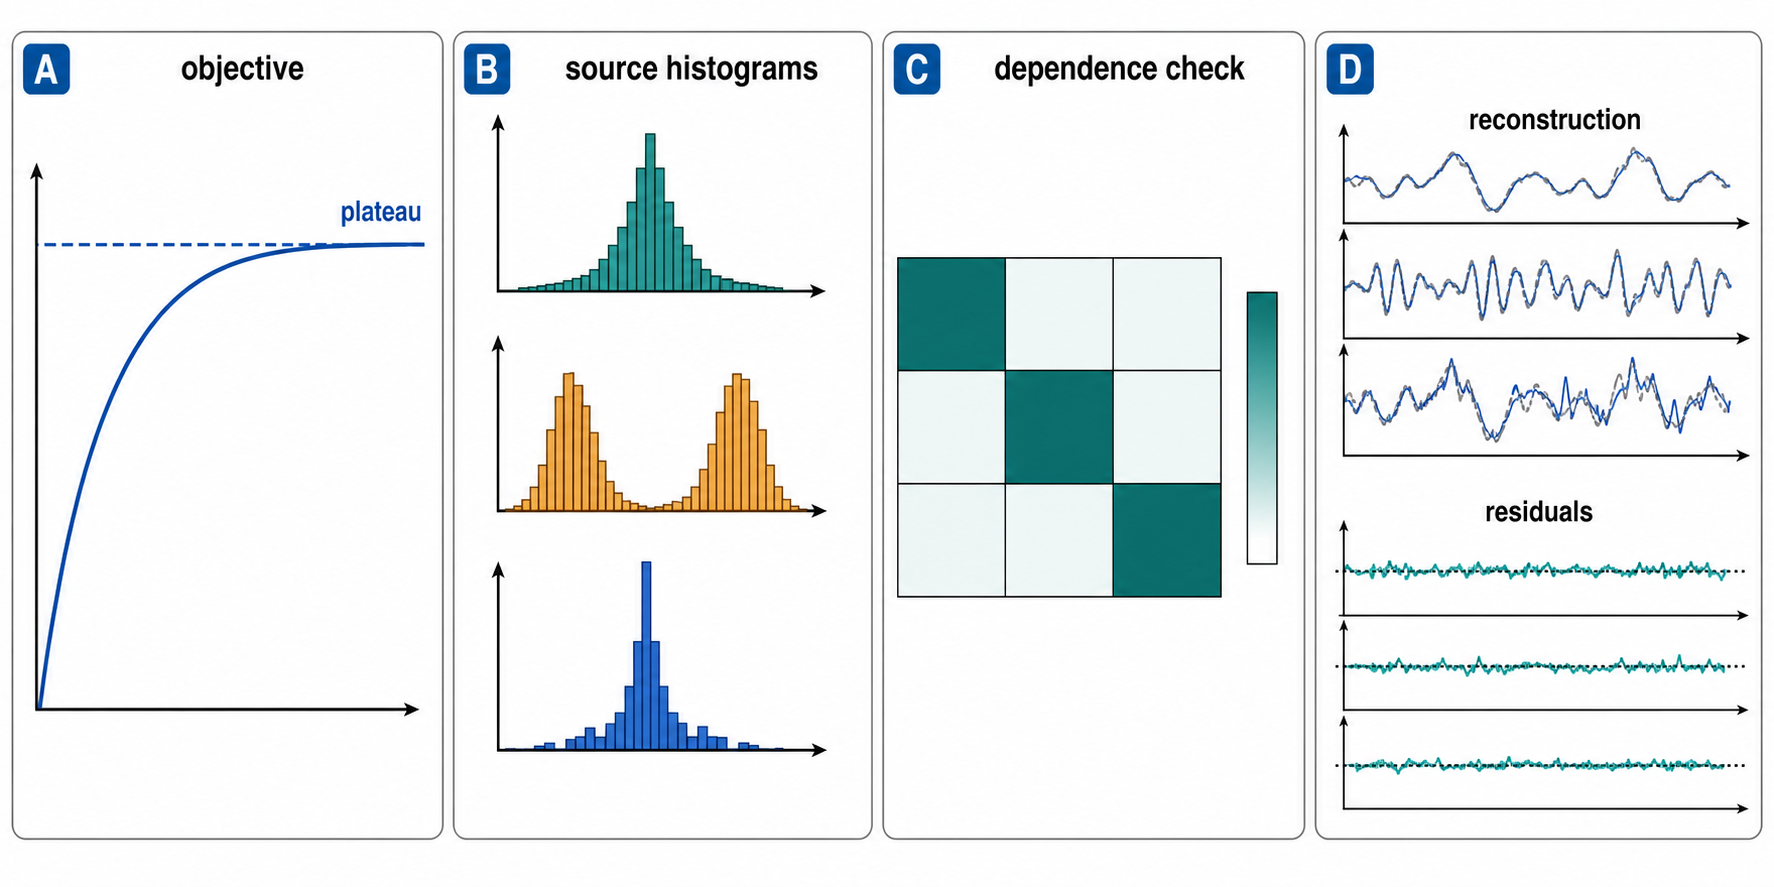
\includegraphics[width=0.96\textwidth]{figures/ica/ica-diagnostics.png}
  \caption{Practical ICA diagnostics. The training objective should stabilize, recovered source histograms should show plausible non-Gaussian structure, dependence between components should be weak, and reconstruction residuals should remain small when the learned unmixing matrix is inverted.}
\end{figure}

\paragraph{Objective trace.}
Track \(E^T(W)\) or its online estimate during learning. It should increase during stable ascent and eventually plateau. Oscillation, divergence, or sudden drops often indicate too large a learning rate, poor conditioning, or a bad nonlinearity for the data.

\paragraph{Whitening spectrum.}
Inspect the eigenvalue spectrum before whitening. Very small eigenvalues make whitening noisy because \(\Lambda^{-1/2}\) amplifies low-variance directions. Truncating tiny eigenvalues can improve stability, but it changes the retained source space.

\paragraph{Residual reconstruction.}
If \(W\) is square and invertible, define \(\hat{A}=W^{-1}\). The reconstruction is
\[
  \hat{x}=\hat{A}\hat{s}=W^{-1}Wx.
\]
For the exact square model this residual should be small:
\[
  r=x-\hat{x}.
\]
A large residual means the implementation or preprocessing is inconsistent, or that the model has been made non-square by dimensionality reduction. In the non-square case, residuals should be interpreted relative to the retained subspace, as in PCA.

\paragraph{Dependence checks.}
Because ICA aims at independence, not just decorrelation, check more than the covariance matrix. Compare component histograms, scatter plots, nonlinear correlations, or estimates of pairwise mutual information. The off-diagonal covariance should be small after whitening, but that alone is not enough.

\paragraph{Component interpretation.}
For EEG-like data, inspect each component's time course, sensor mixing pattern, spectrum, and event relation. ICA separates statistical causes, not automatically biological causes. A component can be a neural signal, an artifact, or a mixture that remains after model mismatch.

\paragraph{Simulation observables.}
In synthetic experiments where \(A\) and \(s\) are known, evaluate
\[
  G = W A.
\]
Successful separation means \(G\) is close to a scaled permutation matrix. This respects the two unavoidable ambiguities: row order and row scale. Directly comparing \(W\) to \(A^{-1}\) without optimizing over those ambiguities is the wrong diagnostic.

\subsection{Summary}

ICA extends the course's projection-method story beyond covariance. The generative model says that observations are linear mixtures \(x=As\) of statistically independent latent sources. PCA and whitening remove mean, covariance, and scale structure, but independence requires using higher-order distributional information. Identifiability is limited by permutation, scale, and Gaussian rotations. Infomax ICA turns independence into an entropy-maximization problem by passing linear source estimates through CDF-like nonlinearities. Gradient and natural-gradient learning then provide online update rules for the unmixing matrix.

The practical lesson is to treat ICA as a latent generative model with diagnostics. Compute the whitening spectrum, monitor the Infomax objective, inspect non-Gaussian marginals and residual dependence, compare \(WA\) to a scaled permutation when ground truth exists, and interpret recovered components only after checking their time courses, spectra, and mixing patterns.
